\tikzset{every picture/.style={line width=0.75pt}} %set default line width to 0.75pt        

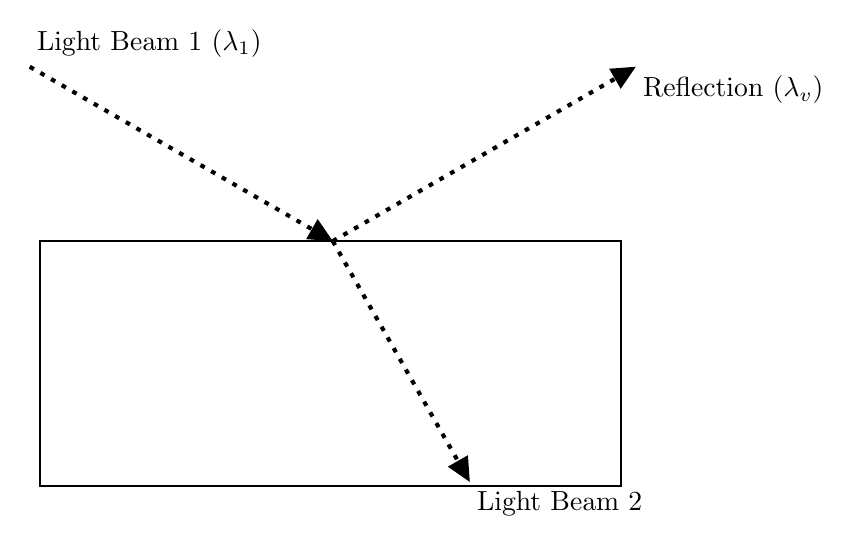
\begin{tikzpicture}[x=0.75pt,y=0.75pt,yscale=-1,xscale=1]
%uncomment if require: \path (0,642); %set diagram left start at 0, and has height of 642

%Shape: Rectangle [id:dp4884979270157479] 
\draw   (152,146) -- (432,146) -- (432,264) -- (152,264) -- cycle ;
%Straight Lines [id:da09234309558155318] 
\draw [line width=1.5]  [dash pattern={on 1.69pt off 2.76pt}]  (147,62) -- (289.53,144.01) ;
\draw [shift={(293,146)}, rotate = 209.91] [fill={rgb, 255:red, 0; green, 0; blue, 0 }  ][line width=0.08]  [draw opacity=0] (11.61,-5.58) -- (0,0) -- (11.61,5.58) -- cycle    ;
%Straight Lines [id:da17812306023892588] 
\draw [line width=1.5]  [dash pattern={on 1.69pt off 2.76pt}]  (293,146) -- (435.53,63.99) ;
\draw [shift={(439,62)}, rotate = 150.09] [fill={rgb, 255:red, 0; green, 0; blue, 0 }  ][line width=0.08]  [draw opacity=0] (11.61,-5.58) -- (0,0) -- (11.61,5.58) -- cycle    ;
%Straight Lines [id:da6647955313115745] 
\draw [line width=1.5]  [dash pattern={on 1.69pt off 2.76pt}]  (293,146) -- (357.02,258.52) ;
\draw [shift={(359,262)}, rotate = 240.36] [fill={rgb, 255:red, 0; green, 0; blue, 0 }  ][line width=0.08]  [draw opacity=0] (11.61,-5.58) -- (0,0) -- (11.61,5.58) -- cycle    ;

% Text Node
\draw (149,59) node [anchor=south west] [inner sep=0.75pt]   [align=left] {Light Beam 1 ($\displaystyle \lambda _{1}$)};
% Text Node
\draw (361,265) node [anchor=north west][inner sep=0.75pt]   [align=left] {Light Beam 2};
% Text Node
\draw (441,65) node [anchor=north west][inner sep=0.75pt]   [align=left] {Reflection ($\displaystyle \lambda _{v}$)};


\end{tikzpicture}
